\documentclass[english]{beamer}

\usepackage[utf8]{inputenc}
\usepackage[T1]{fontenc}
\usepackage{babel}
\usepackage{lmodern}
\usepackage{amsmath, amssymb}
\usepackage{amsfonts}
\usepackage{hyperref}
\usepackage{color}
\usepackage{graphicx}
\graphicspath{ {figures/} }
%\usepackage[left=3cm,right=3cm,top=3cm,bottom=3cm]{geometry}
\usepackage{float}
\usepackage{lmodern} 
\usepackage{xcolor} 
\usepackage{multicol}
%\usepackage[justification=centering]{caption}
\usepackage{caption}
\usepackage{subcaption} 

\setbeamersize{text margin left=0.5cm,text margin right=0.5cm} 

%CHOIX DU THEME et/ou DE SA COULEUR
% => essayer différents thèmes (en décommantant une des trois lignes suivantes)
%\usetheme{PaloAlto}
%\usetheme{Madrid}
% \usetheme{Berlin}
\setbeamertemplate{page number in head/foot}[totalframenumber]
\usetheme{Copenhagen}

% => il est possible, pour un thème donné, de modifier seulement la couleur
%\usecolortheme{crane}
%\usecolortheme{seahorse}
%\usecolortheme{dolphin}
\usecolortheme{seahorse}
\useoutertheme[subsection=false]{smoothbars}

% enlever la barre de navigation
\beamertemplatenavigationsymbolsempty


%Pour le TITLEPAGE
\title[Code-Switching as a Cross-Lingual Training Signal]{Code-Switching as a Cross-Lingual Training Signal: an Example with Unsupervised Bilingual Embedding}
\author[Gaschi et al., 2023 (Mines Nancy - LORIA - POSOS)]{\small Félix Gaschi$^{2,3}$, Ilias El Baamarani$^1$, Barbara Gendron$^1$, Parisa Rastin$^2$, Yannick Toussaint$^2$}
\date{3rd Multilingual Representation Learning Workshop @ EMNLP 2023}
\institute[Mines Nancy - LORIA - POSOS]{\scriptsize $^1$École des Mines de Nancy, $^2$LORIA, $^3$SAS Posos}

\begin{document}


\begin{frame}
	\begin{figure} 
	\hspace*{0.5cm}
	\begin{minipage}[c]{.20\linewidth} 
	
\includegraphics[scale=0.04]{Logo_Mines_Nancy.png} 
	\end{minipage} \hfill 
	\begin{minipage}[c]{.40\linewidth} 
	
\includegraphics[scale=0.06]{posos.png} 
	\end{minipage} 
    \begin{minipage}[c]{.20\linewidth} 
        
\includegraphics[scale=0.15]{loria.png} 
    \end{minipage} 
	\end{figure}
	\titlepage
	
\end{frame}

\section{Introduction}

\begin{frame}{Code-Switching (CS)}
	Code-switching (CS): words from \textbf{different languages} are found in the \textbf{same sentence}.\\
	\vspace*{0.5cm}
	Language contamination (LC): \textbf{whole sentences} from other languages in a monolingual corpus.
	\visible<2->{
	\begin{itemize}
		\item<3->[($+$)] Always present in (supposedly) monolingual corpora~{\footnotesize [Blevins and Zettlemoyer, 2022]}
		\item<4->[($+$)] Support for cross-lingual generalization abilities in monolingual embeddings
		\item<5->[($-$)] No context sharing because no token/sentence pairs  
	\end{itemize}}
	% CS vs language contamination
	% Language contamination always present, therefore already used (Language contamination is already a support for cross-lingual generalization abilities in monoligual embeddings)
	% CS a l'avantage de proposer des paires de tokens qui partagent le même contexte
	% On va leverage CS pour apprendre des embeddings statiques bilingues
\end{frame}

\begin{frame}{CS in monolingual corpora}
	\begin{figure}
		\centering
		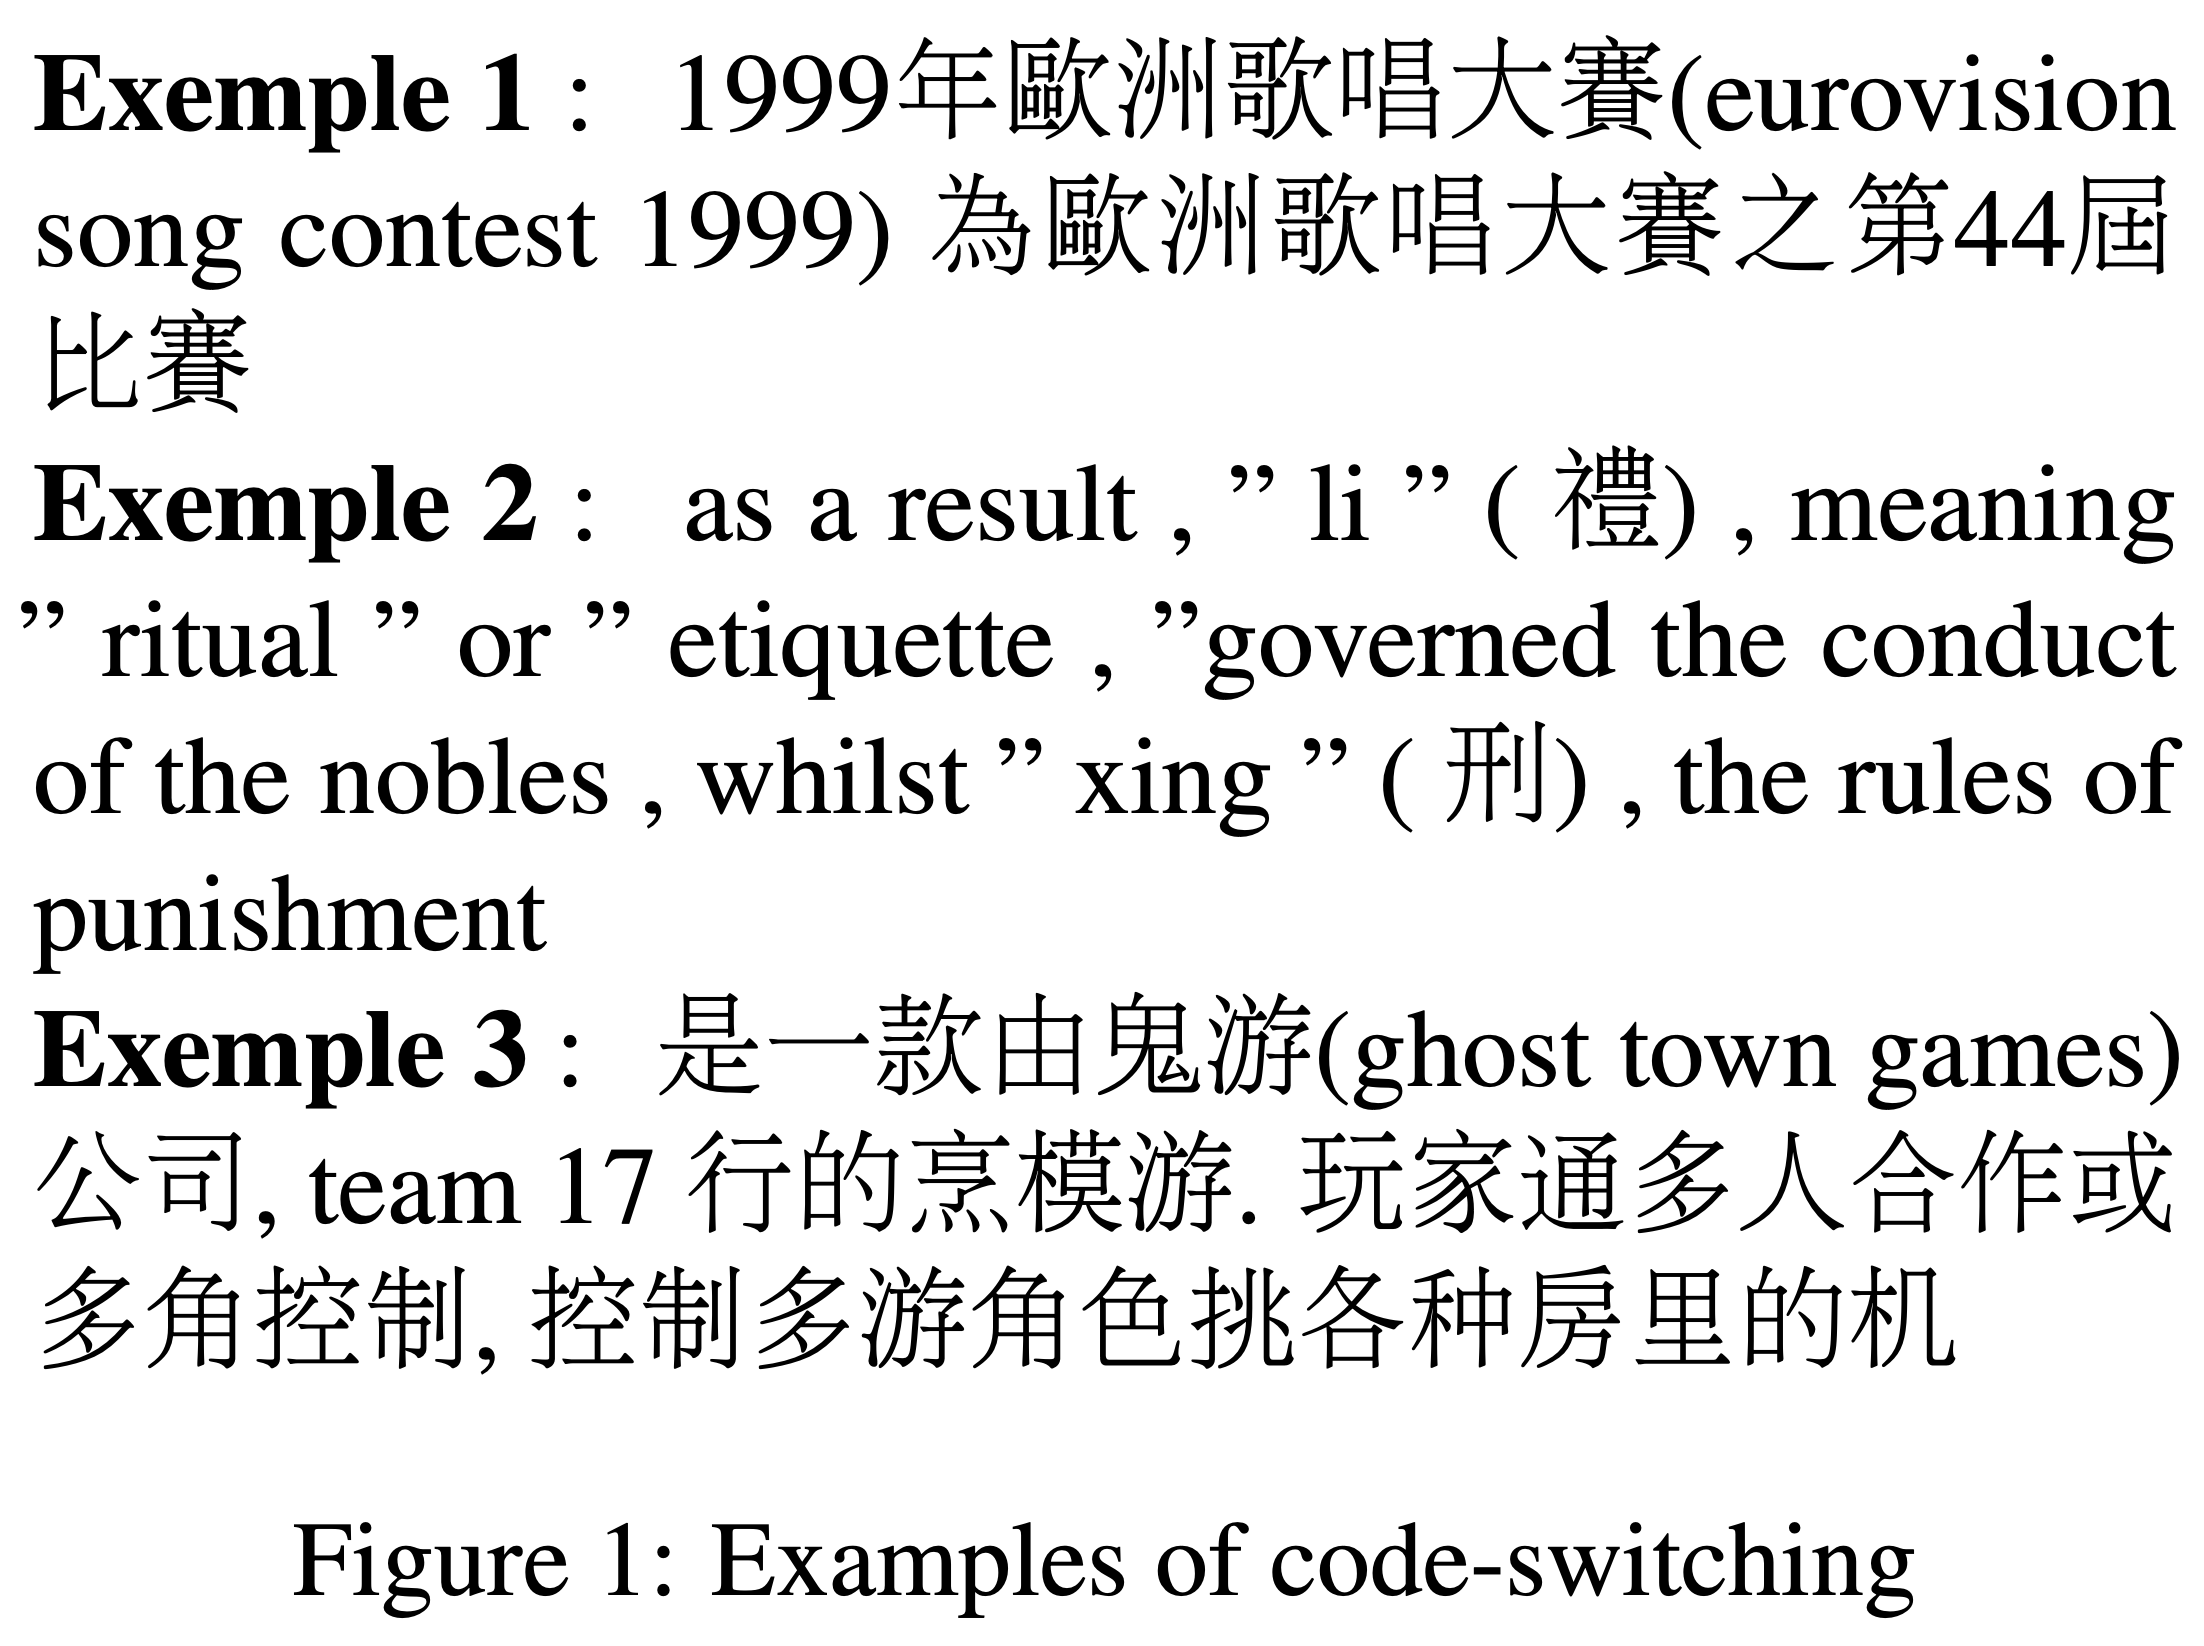
\includegraphics[width=0.70\textwidth]{cs-example.png}
	\end{figure}
\end{frame}

\section{Related work}

\begin{frame}{Cross-lingual embeddings}
Trade-off required ressources / alignment robustness:
	\begin{itemize}
		\item Supervised methods: BDI requires parallel corpora~{\footnotesize [Mikolov et al., 2013]}
		\item Fully unsupervised embedding alignment~{\footnotesize [Conneau et al., 2017]} often lacks of robustness~{\footnotesize [Søgaard et al., 2018]}
		\item A weak supervision signal brings more stability~{\footnotesize [Søgaard et al., 2018]}
	\end{itemize}
\vspace*{1.5cm}
\visible<2->{\textcolor{blue}{$\longrightarrow$ CS would act as a weak supervision signal bilingual embedding learning.}}
\end{frame}

\begin{frame}{CS-enhanced cross-lingual embedding learning}
	CS-powered cross-lingual mappings: \textbf{tokens randomly replaced by their translation}. 
	% This should be equivalent to any mapping-based method.
	\begin{itemize}
		\item Alleviate the amount of parallel data~{\footnotesize [Krishnan et al., 2021]}
		\item Improve PLMs' cross-lingual generalization~{\footnotesize [Qin et al., 2020, Yang et al., 2020]}
	\end{itemize}
	$\longrightarrow$ Artificially-generated CS\\
	\vspace*{0.5cm}
	\visible<2->{
	Ours:
	\begin{itemize}
		\item[(1)] Identifies CS situations in monolingual corpora
		\item[(2)] Uses \textbf{natural CS} to learn a bilingual embedding using orthogonal mapping across languages
	\end{itemize}}
	
\end{frame}

\section{Methodology}

\begin{frame}{Code-switching identfication}
\textcolor{blue}{No supervision: don't want to rely on a full bilingual dictionnary!}\\
$\longrightarrow$ Use \textbf{regular expressions} to detect CS situations.
\vspace*{0.5cm}\\
\visible<2->{
	Consequences:
	\begin{itemize}
		\item Scope reduction: languages written in different scripts\\ (en-zh, en-ru, en-ar)
		\item Code-switching detection $\rightarrow$ script-switching detection?
	\end{itemize}
}
\vspace*{0.5cm}
\visible<3->{
	Code-switching pair: pair of words from different scripts found \textbf{in the same context window}.
}
\end{frame}

\begin{frame}{Training procedure}
	Based on monolingual skip-gram loss~{\footnotesize [Mikolov et al., 2013]}:
\begin{equation}
	L = - \frac{1}{|C|} \sum_{w_i \in C} \sum_{w_j \in \mathcal{N}(w_i)} \textcolor{blue}{\log P(w_j | w_i)}
\end{equation}
\visible<2->{
Replace the original negative sampling:
\begin{equation}
		\textcolor{blue}{\log P(w_j | w_i)} = \log \sigma(\tilde{x}_{j}^\top \textcolor<3->{purple}{x_{i}}) + \sum_{w_k\sim P_V}^{n}\log \sigma(-\tilde{x}_{k}^\top \textcolor<3->{purple}{x_{i}})
\end{equation}
}
\visible<3->{
By computation on projected tokens in a CS pair $(w_i^{src}, w_j^{tgt})$:
\begin{equation}
		\textcolor{blue}{\log P(w^\text{tgt}_j | w^\text{src}_i)} =  \log \sigma({{\tilde{x}}^\text{tgt}_j}\,^\top \textcolor{purple}{W x_i^\text{src}}) + \sum_{w^\text{tgt}_k\sim \mathcal{U}_{V_\text{tgt}}}^{n}\log \sigma(-\tilde{x}^\text{tgt}_{k}\,^\top \textcolor{purple}{W x^\text{src}_i})
\end{equation}
}
\end{frame}

\begin{frame}{Experimental setup}
CS pairs extraction:
\begin{itemize}
	\item Data is tokenized Wikipedia dumps 
	\item FastText~{\footnotesize [Bojanowski et al., 2016]} monolingual embeddings for 200,000 most frequent words
	\item Context window of width 5
\end{itemize}
\vspace*{0.5cm}
\visible<2->{
Training pipeline:
	\begin{itemize}
		\item Modified skip-gram loss for \textbf{model initialisation}
		\item Add \textbf{orthogonalization steps} so $W$ preserves distances
		\item \textbf{Refinement step} using \texttt{VecMap} self-learning procedure~{\footnotesize [Artetxe et al., 2018]}
	\end{itemize}
}
\end{frame}

\section{Results}

\begin{frame}{Code-switching in monolingual corpora}
	\begin{columns}
	\begin{column}{0.45\linewidth}
		\begin{itemize}
			\item Check for script-switching with a dictionnary
			\item Differentiate CS and token contamination
		\end{itemize}
	\end{column}
	\begin{column}{0.45\linewidth}
		\begin{figure}
			\centering
			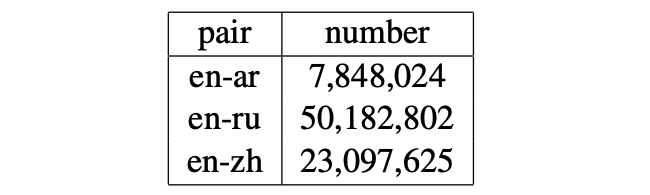
\includegraphics[width=\textwidth]{cs-pairs.png}
			\caption{\centering Counts of CS pairs}
		\end{figure}
	\end{column}
	\end{columns}

	\begin{figure}
		\centering
		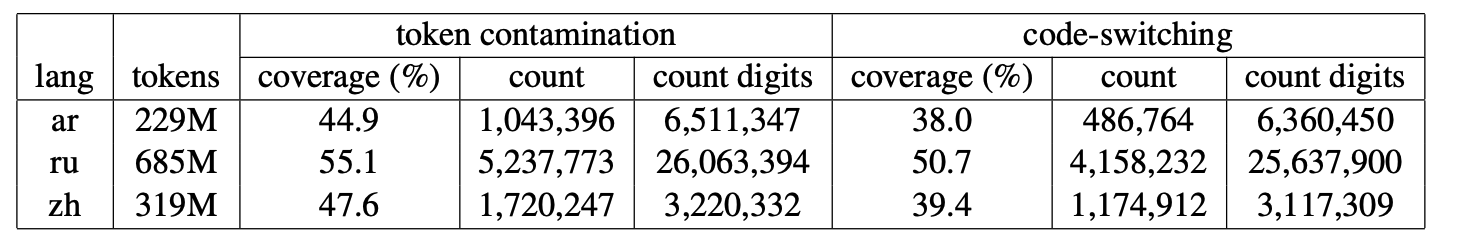
\includegraphics[width=\textwidth]{results.png}
		\caption{\centering Presence of English words in non-English monolingual corpora. An example is considered code-switched if it is in the vicinity of a non-English word.}
	\end{figure}
\end{frame}

\begin{frame}{Results of \texttt{CoSwitchMap}}
	\begin{figure}
		\centering
		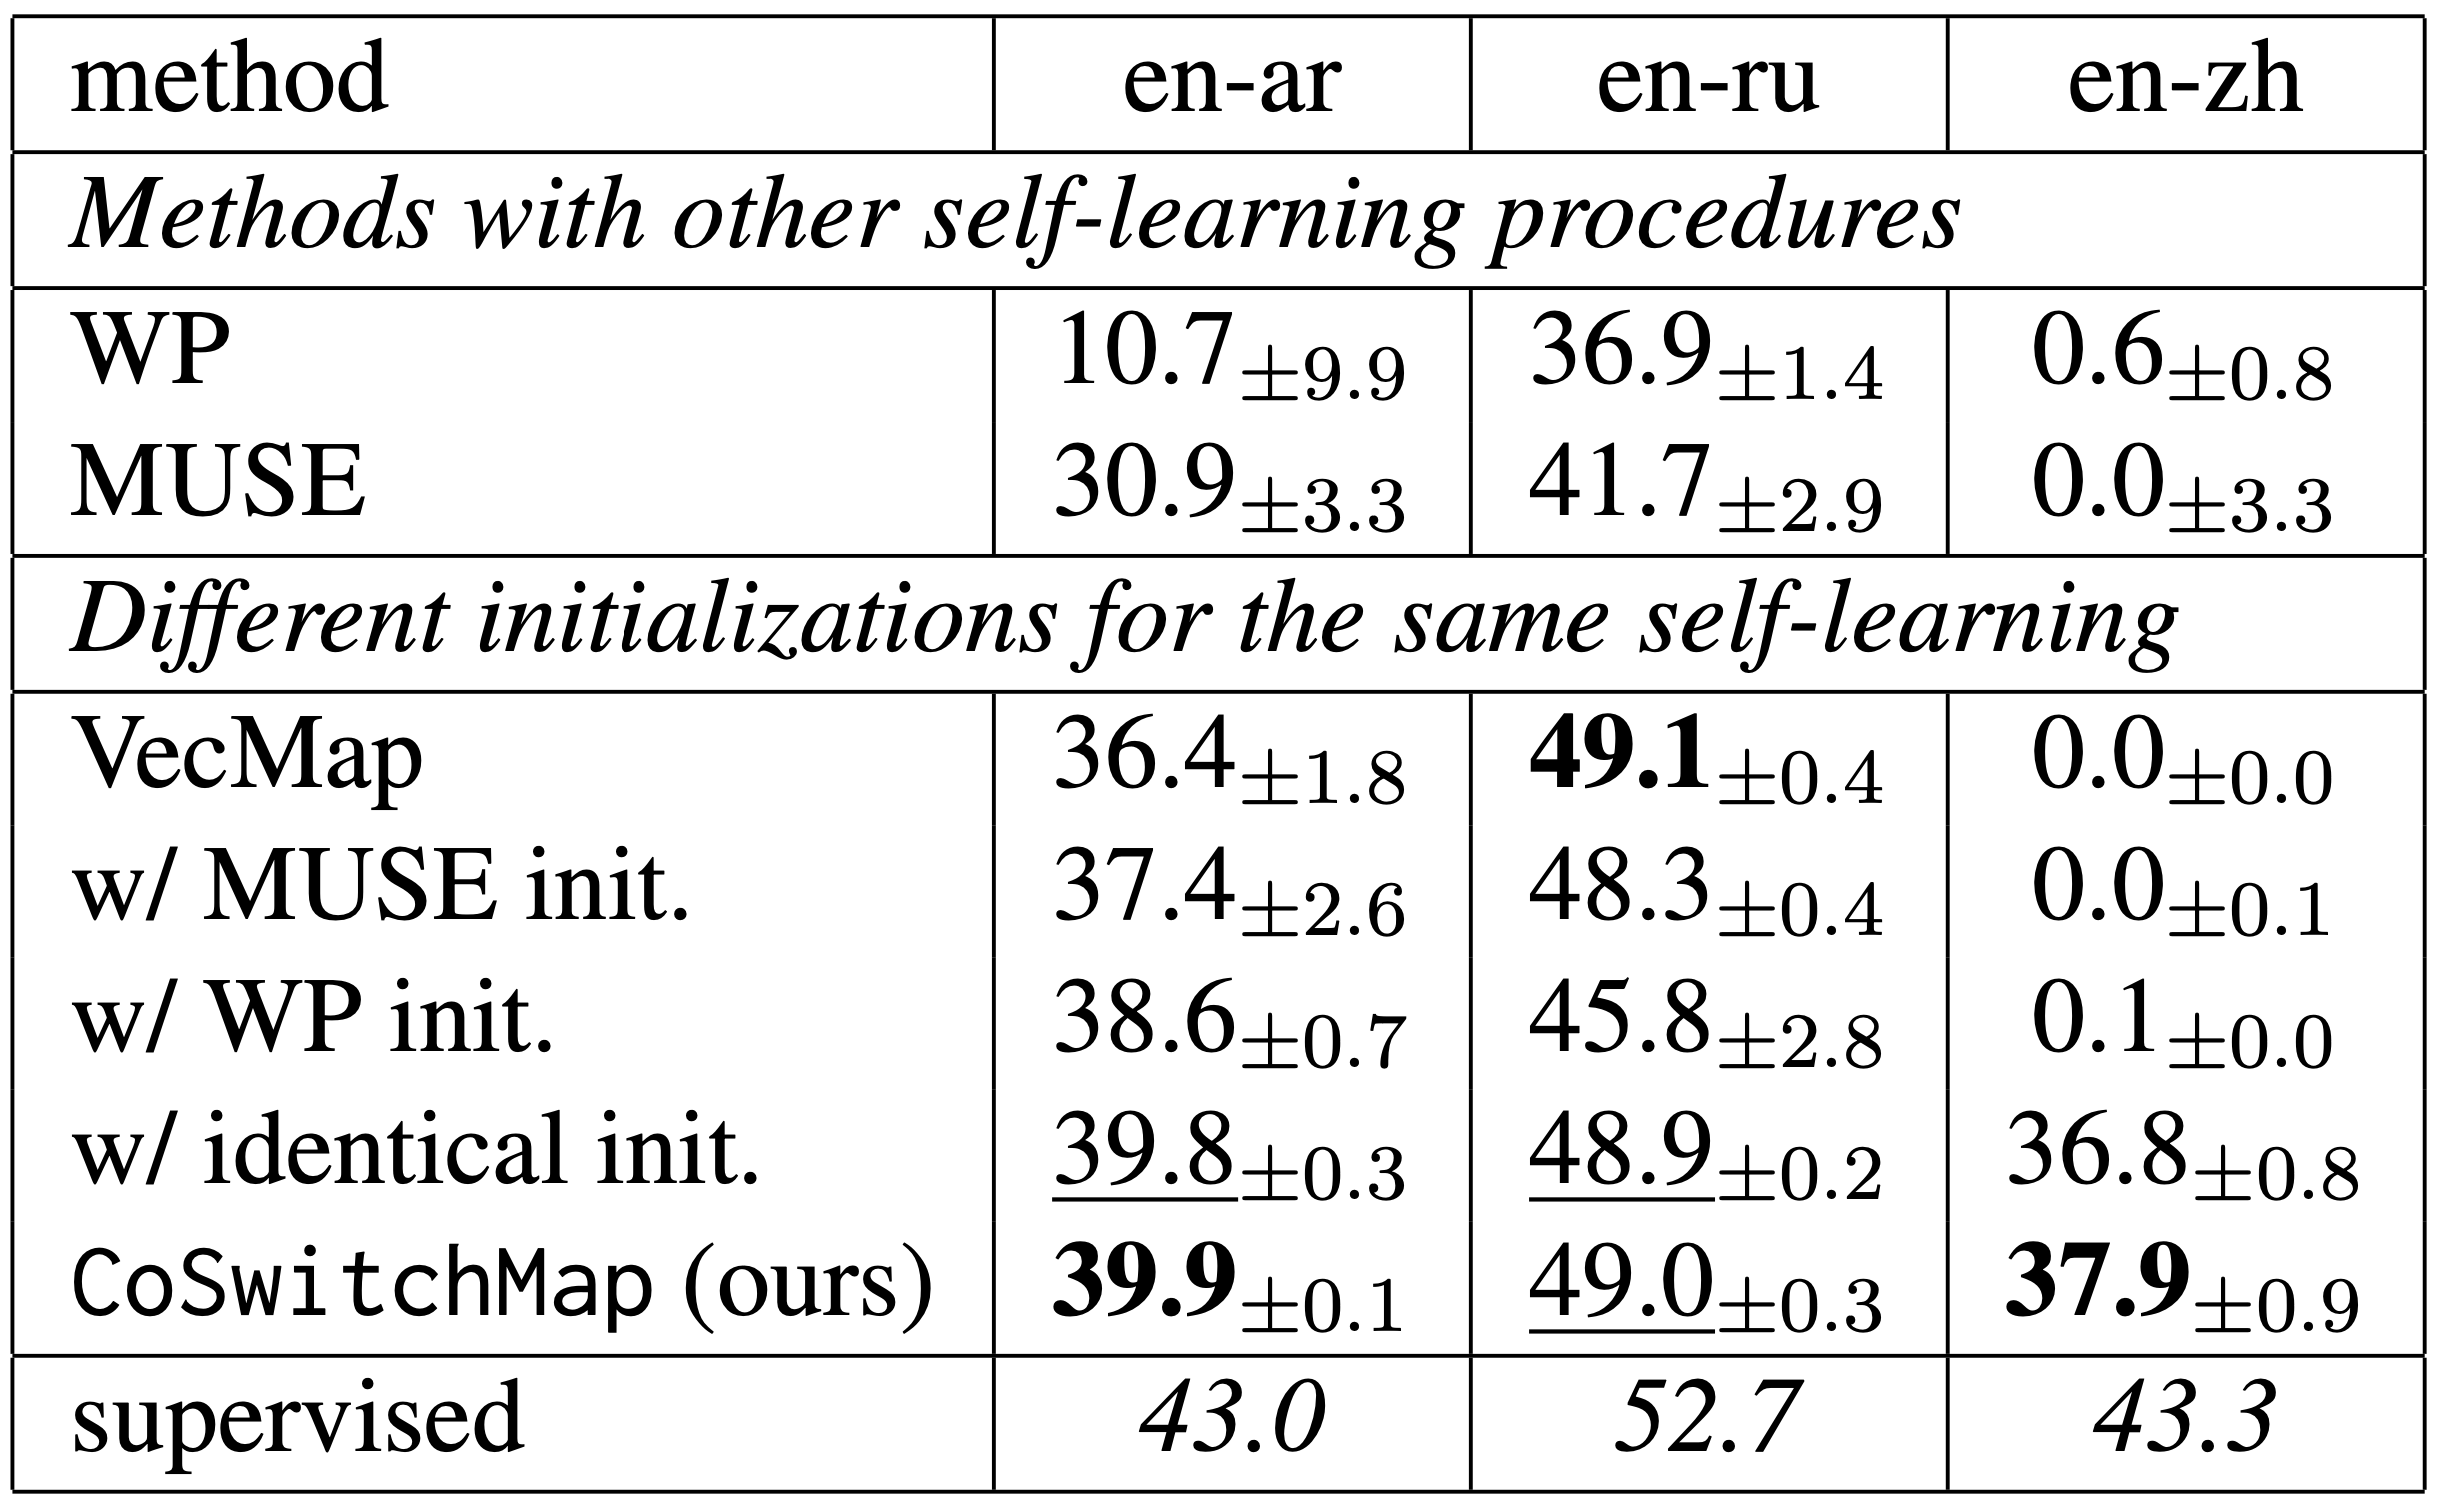
\includegraphics[width=0.80\textwidth]{results-coswitchmap.png}
		\caption{\centering Comparison of \texttt{CoSwitchMap} with other unsupervised mapping-based methods. Top-1 accuracy of a nearest neighbout search with CSLS criterion for BLI.}
	\end{figure}
\end{frame}

\section{Conclusion}

\begin{frame}{Conclusion}
Contributions:
	\begin{itemize}
		\item \texttt{CoSwitchMap} outperforms existing unsupervised mapping-based methods
		\item Natural CS constitutes a cross-lingual training signal for multilingual static embeddings
		\item Leverage naturally-occuring code-switching 
	\end{itemize}
\vspace*{0.3cm}
\visible<2->{
Limitations:
\begin{itemize}
	\item Only works with languages written in different scripts. % Specificity of method
	\item Most of the CS situations are litteral translations of words in the vicinity. % Specificity of data
	\item Demonstrates the utility of code-switching but still need for a more generalized method.
\end{itemize}}
\end{frame}

\appendix

\begin{frame}[allowframebreaks]{References}

\begin{thebibliography}{9}

	% Artificially induced CS (1)
	\bibitem[Xiao and Guo, 2014]{xg2014}
	Min Xiao and Yuhong Guo (2014). \emph{Distributed word representation learning for cross-lingual dependency parsing.} CoNLL 2014.
	
	% Artificially induced CS (2)
	\bibitem[Gouws and Søgaard, 2015]{gs2015}
	Gouws and Søgaard (2015). \emph{Simple task-specific bilingual word embeddings}. EMNLP 2018.

	% BDI
	\bibitem[Mikolov et al., 2013]{mikolov2013}
	Mikolov et al. (2013). \emph{Exploiting similarities among languages for machine
	translation}. CoRR, abs/1309.4168.

	% Unsupervised cross-lingual embeddings
	\bibitem[Conneau et al., 2017]{conneau2017}
	Conneau et al. (2017). \emph{Word translation withour parallel data}. ICLR 2018.

	% Limitations
	\bibitem[Søgaard et al., 2018]{sogaard2018}
	Søgaard et al. (2018). \emph{On the limitations of unsupervised bilingual dictionary induction}. ACL 2018.

	% CS to improve PLMs (1)
	\bibitem[Qin et al., 2020]{qin2020}
	Qin et al. (2020). \emph{Cosda-ml: Multi-lingual code-switching data augmentation for zero-shot cross-lingual NLP}. IJCAI 2020.

	% CS to improve PLMs (2)
	\bibitem[Yang et al., 2020]{yang2020}
	Yang et al. (2020). \emph{Alternating language modeling for cross-lingual pre-training}. AAAI 2020.


	% CS to improve PLMs (2)
	\bibitem[Artetxe et al., 2018]{artetxe2018}
	Artetxe et al. (2018). \emph{A robust self-learning method for fully unsupervised cross-lingual mappings of word embeddings}. ACL 2018.

	\end{thebibliography}	
	
\end{frame}

\end{document}